\section{Procedimento \& Analisi dati}

\subsection{Relazione tra l'indice di rifrazione di un materiale e la lunghezza d'onda del raggio incidente}

La prima operazione eseguita è stata quella di misurare l'angolo ''zero''. Ovvero abbiamo misurato l'anglolo segnato dal goniometro quando tra la sorgente luminosa e il canocchiale, allineati, non vi era interposto alcun'oggetto. Ricordiamo che più si stringe la fenditura del collimatore più la misura dell'angolo ''zero'' risulta essere precisa. Questo compatibilmente con l'intensità luminosa osservabile da un occhio umano.
L'angolo ''zero'' quindi ha il seguente valore:

\begin{equation}
	\theta\ped{0} \,=\, 128^\circ \,31' \pm 1'
\end{equation} 

Ora vogliomo osservare la relazione che sussiste tra l'indice di rifrazione del nostro prisma di vetro e la lunghezza d'ona di un raggio luminoso.
A tal fine occorre ricordare che un raggio luminoso incidente su una faccia di un prisma subisce una riflessione e una rifrazione, poichè passa da un mezzo ad un altro.
Consideriamo ora cosa accade al raggio rifratto. Poichè il raggio luminoso incidente non è monocromatico questo è composto da numerosi raggi luminosi con lunghezza d'onda differente, tutte quelle presenti nello spettro del visibile. Infatti quando il raggio incidente viaggia attraverso il prisma si scompone nelle sue varie componenti (dispersione della luce) a seconda delle diffrenti lunghezze d'onda che lo comongono. Quindi i ragi monocromatici subiscono un'ulteriore rifrazione passando nuovamente dal vetro all'aria, uscendo pertanto dal prisma. Questa seconda rifrazione non porta altro che ad un'amplificazione dell'effetto precedente, pertanto è più semplice distinguere i vari raggi luminosi.
In questa esperienza noi non siamo in grado di misurare direttamente la lunghezza d'onda di un raggio luminoso. Ciononostante sappiamo che ad un dato colore del raggio luminoso corrisponde una certa lunghezza d'onda, pertanto ci interessa trovare l'indice di rifrazione, del prisma, corrispondente ai nostri raggi monocromatici e quindi ad una precisa lunghezza d'onda ($\lambda$).
A tal fine noi sappiamo che, in un prisma, per ottenere l'indice di rifrazione di un materiale senza conoscere la lunghezza d'onda del raggio luminoso incidente, basta conoscere l'angolo massimo ($\theta\ped{max}$) di uscita del raggio rifratto rispetto al proungamento della direzione incidente. Quindi noto questo valore applichiamo la sguente relazione:

\begin{equation}
	n \,=\, \frac{\sin{(\alpha\,+\,\frac{\theta\ped{max}}{2})}}{\sin{\frac{\alpha}{2}}}
	\label{indice_rif}
\end{equation}

dove $\alpha$ è l'angolo di apertura del prisma, che nel nostro caso vale $60^\circ$, e ci ricaviamo così il valore dell'indice di rifrazione in base al colore (quindi indirettamente alla lunghezza d'onda) del raggio luminoso in esame.
Per completare il quadro teorico è doveroso chiarire cosa si ntenda con $\theta\ped{max}$: questo angolo è l'angolo massimo di uscita, dal prisma, del ragio monocromatico. Infatti sperimentalmente si è osservato che sopra un certo $\theta$ il raggio luminoso non continua ad aumetare l'angolo che forma con il prolungamento del raggio incidente, ma ''ritorna indietro''.\\
%scusatemi, questa ultima descrizione non sono riuscito a farla meglio. Lo so Pasa mi vuole ammazzare perchè tocca fare tutto a lui... :(

Ora questa è la teoria che stà alla base dell'esperienza. Operativamente per misurare $\theta\ped{max}$ abbiamo adottato la seguente procedura:

\begin{itemize}
	\item{si posiziona il prisma al centro del goniometro. Successivamente si ruota il prisma per cercare di ottenere $\theta\ped{max}$, aiutandosi con il canocchiale;}
	\item{una volta ottenuto $\theta\ped{max}$ si cerca di allineare il meglio possibile il canocchiale col crocifilo con il raggio monocromatico in esame e si legge sullo spettrogoniometro il valore dell'angolo segnato ($\theta\ped{i}$);}
	\item{quindi per ottenere $\theta\ped{max}$ non si deve fare altro che una semplice differenza tra $\theta\ped{i}$ e $\theta\ped{0}$;}
\end{itemize}

Infine una volta ottenuti i vari valori di $\theta\ped{max}$ per ciascuno dei raggi monocromatici che siamo stati in grado di distinguere ne calcoliamo il rispettivo indice di rifrazione sfruttando la relazione (\ref{indice_rif}). I valori che abbiamo ottenuto sono riportati nella seguente tabella, nella quale è stato associato al colore del raggio monocromatico la ripettiva lunghezza d'onda, ottenuta trammite supporto multimediale.

\begin{table}[H]
    \centering
    \small
    \begin{tabular}{l c c}
        \toprule
        Colore & $\theta\ped{max}$ & $n \pm dn$ \\
        \midrule
		Rosso 1	& 	$167^\circ \, 00' \pm 1'$ &	$1.5149 \pm 0.0003$ \\	
		Rosso 2	& 	$167^\circ \, 02' \pm 1'$ &	$1.5153 \pm 0.0003$ \\
		Rosso 3	& 	$167^\circ \, 05' \pm 1'$ &	$1.5159 \pm 0.0003$ \\
		Verde &		$167^\circ \, 32' \pm 1'$ &	$1.5210 \pm 0.0003$ \\
		Blu &		$167^\circ \, 42' \pm 1'$ &	$1.5229 \pm 0.0003$ \\
		Viola &		$167^\circ \, 47' \pm 1'$ &	$1.5238 \pm 0.0003$ \\
        \bottomrule
    \end{tabular}
    \caption{Dati relativi all'indice di rifrazioe $n$ in funzione del colore e quindi della lunghezza d'onda $\lambda$.}
    \label{tab:enne}
\end{table}


Come possiamo notare dai valori tabulati l'indice di rifrazione dei vari raggi monocromatici verde blu e viola varia solo se si osserva la terza cifra decimale, mentre tra questi e il rosso la diffrenza la si può notare anche esaminando la seconda cifra decimale. Questa differenza ha senso perchè osservando la distanza, tra loro, dei raggi con il canocchiale, il raggio monocromatico rosso era sensibilmente più distante dagli altri raggi, come si può notare anche dai rispettivi valori di lunghezza d'onda. Infatti il raggio di colore rosso si trova ad un estremo dello spettro del visibile, mentre i raggi verde blu e viola sono più vicini all'altra estremità dello spettro luminoso visibile, ovvero dalla parte del colore blu/viola. Infine sperimentalmente abbiamo avuto non poche difficoltà ad individuare le due gradazioni di rosso oltre a quella primaria. Questa difficoltà si può comprendere se si osserva che l'indice di rifraione per i tre raggi monocromatici rossi varia soltanto attorno alla quarta cifra decimale. Inoltre anche le rispettive lunghezze d'onda non sono poi così marcatamente differenti.

\subsection{Verifica sperimentale della legge che lega l'angolo di incidenza, sul prisma, di un raggio luminoso col relativo angolo di uscita}

In questa seconda parte dell'esperienza vogliamo verificare la seguente relazione sperimentale:

\begin{equation}
	\theta \,=\, \arcsin{(n - \sin{r})} + \arcsin{(n \, \sin{(\alpha - r)})} - \alpha
	\label{eq:brutta}
\end{equation}

dove: $\theta$ indica l'angolo che ha il raggio monocromatico uscente dal prisma rispetto al prolungamento del raggio incidente, $\alpha$ non è altro che l'angolo di apertura del prisma, e $r$, rappresenta l'angolo di rifrazione interno al prisma, ovvero l'angolo del raggio rifratto rispetto alla perpendicolare. Infatti il suo valore è immediatamente ricavabile dalla legge di Snell:

\begin{equation}
	 n\ped{i} \, \sin{\theta\ped{i}} = n\ped{r} \, \sin{r}
	 \label{snell}
\end{equation}

dove $n_i$ rappresenta l'indice di rifrazione dell'aria, mentre $n_r$ rappresenta l'indice di rifrazione che assume il materiale a seconda del raggio considerato in quanto il valore di $n_r$ varia a seconda della lunghezza d'onda ($\lambda$) del raggio in esame. Ricordiamo che i valori di $n_r$ in relazione a $\lambda$ sono stati ricavati nella prima parte dell'esperienza. Infine $\theta\ped{i}$ rappresenta l'angolo di incidenza del raggio luminoso sulla faccia del prisma.
Quindi usando $r$ come variabile e conoscendo, per misura diretta $\theta\ped{i}$, posso ricavare $\theta$ dalla (\ref{eq:brutta}).

Pertanto quello che dobbiamo fare, in pratica, è misurare $\theta\ped{i}$ col seguente procedimento:

\begin{itemize}
	\item{abbiamo scelto di ricavare $\theta$ per il raggio monocromatico di colore verde, quindi di lunghezza d'onda pari a XXX;}
	\item{non potendo tuttavia misurare direttamente l'angolo di incidenza ($\theta\ped{i}$) abbiamo misurato l'angolo di riflessione del raggio riflesso allineando il canocchiale col crocifilo la raggio riflesso. Quindi sapendo che l'angolo di incidenza non è altro che la metà dell'angolo misurato abbiamo trovato $\theta\ped{i}$;}
	\item{quindi per ognuno dei 23 angoli di incidenza misurati abbiamo preso il corrispettivo valore di $\theta$ allineando il canocchiale col crocifilo con il raggio monocromatico verede uscente al prisma;}
	\item{infine confronteremo i $\theta$ sperimentali con i valori trovati grazie alla relazione (\ref{eq:brutta}) e scoprimemo pertanto se quest'utima è una relazione valida;}
\end{itemize}

Come si può osservare dal grafico infigura (\ref{fig:dev}) abbimo ottenuto dei dati che combaciano molto bene con la legge sperimentale (\ref{eq:brutta}) in esame, tralasciando due punti, che con molta probabilità non sono stati presi accuratamente come gli altri. Quindi ci sentiamo di dire che la relazione (\ref{eq:brutta}) che lega $\theta$ con l'angolo di incidenza del raggio luminoso sulla faccia del prisma è verificata.

\begin{figure}[b]
    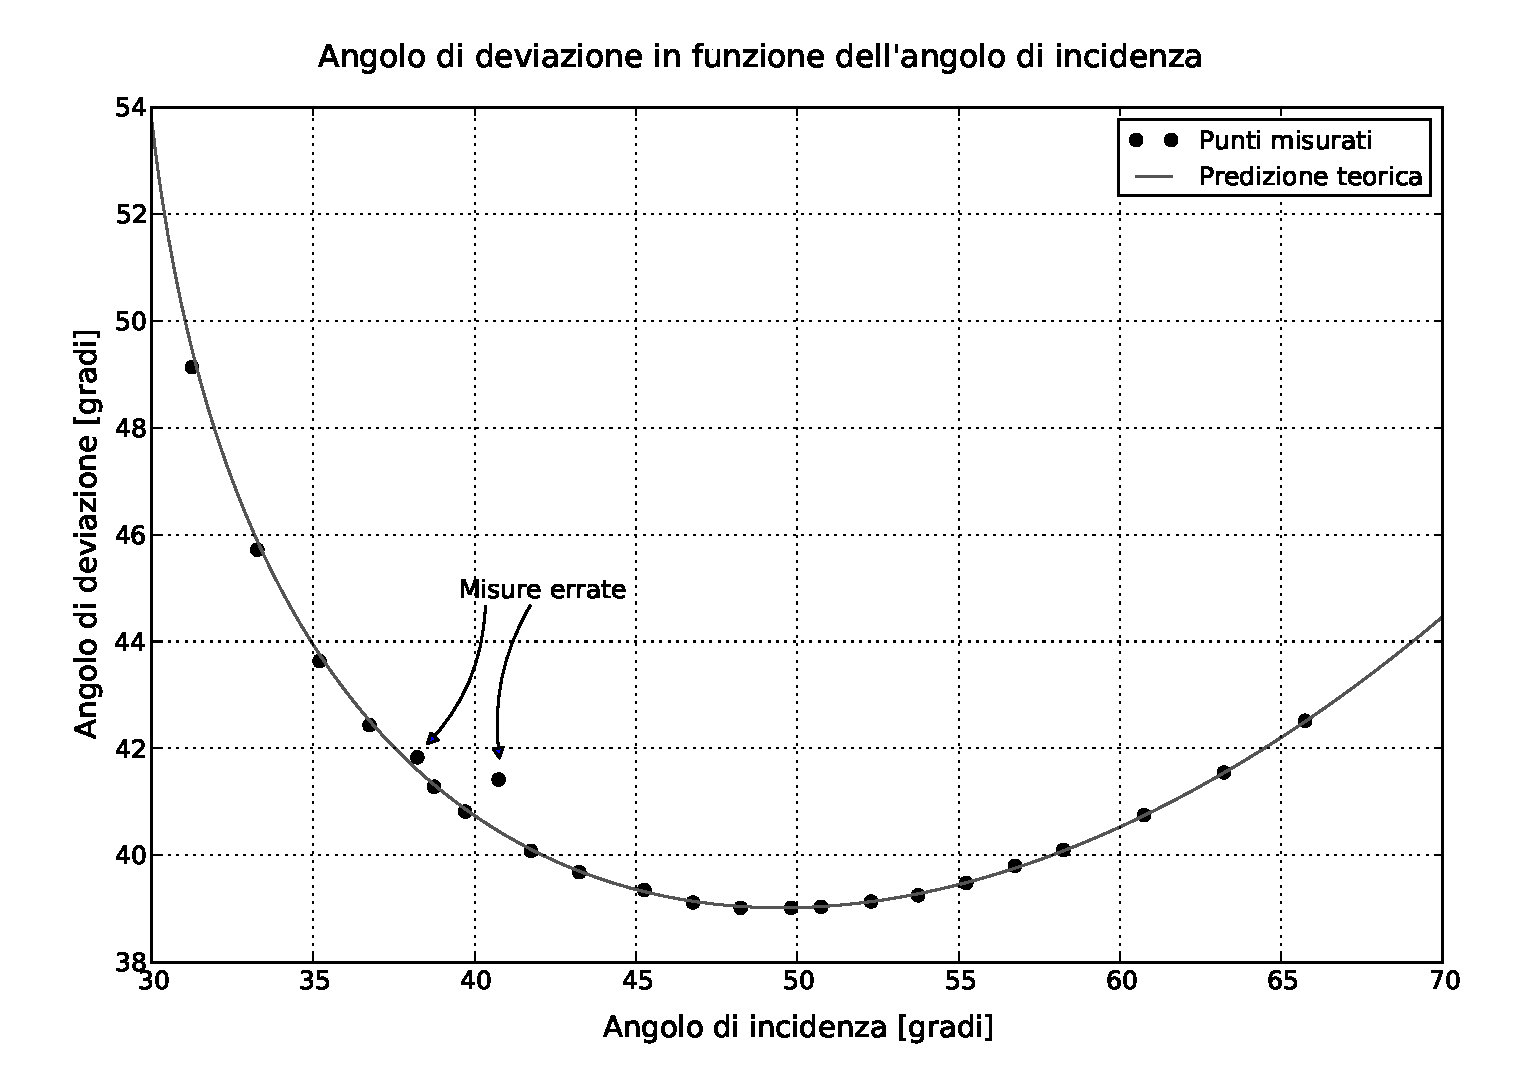
\includegraphics[width=16cm]{graph.pdf}
    \caption{Il grafico mostra i punti che abbiamo raccolto assieme ad un plot della legge (\ref{eq:brutta}). I dati concordano
    molto bene con la curva teorica, sebbene ci siano due punti errati, sicuramente dovuti ad errori nelle misure. L'errore di
    risoluzione è piccolo e non è mostrato in figura, in quanto le barre d'errore sono invisibili.}
    \label{fig:dev}
\end{figure}

\begin{table}[H]
    \centering
    \small
    \begin{tabular}{c c}
        \toprule
	$\theta\ped{i}$ & $\theta$ \\
        \midrule
	$31^\circ \, 15' \pm 1'$ &	$49^\circ \, 15' \pm 4'$ \\	% 31.145   49.280
	$33^\circ \, 16' \pm 1'$ &	$45^\circ \, 16' \pm 4'$ \\	% 33.160   45.528
	$35^\circ \, 12' \pm 1'$ &	$43^\circ \, 12' \pm 4'$ \\	% 35.115   43.456
	$36^\circ \, 44' \pm 1'$ &	$42^\circ \, 45' \pm 4'$ \\	% 36.445   42.312
	$38^\circ \, 14' \pm 1'$ &	$41^\circ \, 14' \pm 4'$ \\	% 38.135   41.358
	$38^\circ \, 45' \pm 1'$ &	$41^\circ \, 45' \pm 4'$ \\	% 38.445   41.193
	$39^\circ \, 43' \pm 1'$ &	$40^\circ \, 43' \pm 4'$ \\	% 39.425   40.520
	$40^\circ \, 45' \pm 1'$ &	$40^\circ \, 45' \pm 4'$ \\	% 40.445   40.270
	$41^\circ \, 45' \pm 1'$ &	$40^\circ \, 45' \pm 4'$ \\	% 41.445   40.067
	$43^\circ \, 15' \pm 1'$ &	$39^\circ \, 15' \pm 4'$ \\	% 43.145   39.421
	$45^\circ \, 16' \pm 1'$ &	$39^\circ \, 16' \pm 4'$ \\	% 45.155   39.191
	$46^\circ \, 46' \pm 1'$ &	$39^\circ \, 46' \pm 4'$ \\	% 46.460   39.083
	$48^\circ \, 15' \pm 1'$ &	$39^\circ \, 15' \pm 4'$ \\	% 48.145   39.025
	$49^\circ \, 49' \pm 1'$ &	$39^\circ \, 49' \pm 4'$ \\	% 49.485   39.011
	$50^\circ \, 44' \pm 1'$ &	$39^\circ \, 44' \pm 4'$ \\	% 50.440   39.024
	$52^\circ \, 17' \pm 1'$ &	$39^\circ \, 17' \pm 4'$ \\	% 52.170   39.079
	$53^\circ \, 45' \pm 1'$ &	$39^\circ \, 45' \pm 4'$ \\	% 53.445   39.167
	$55^\circ \, 14' \pm 1'$ &	$39^\circ \, 14' \pm 4'$ \\	% 55.140   39.293
	$56^\circ \, 45' \pm 1'$ &	$39^\circ \, 45' \pm 4'$ \\	% 56.445   39.454
	$58^\circ \, 15' \pm 1'$ &	$40^\circ \, 15' \pm 4'$ \\	% 58.145   40.048
	$60^\circ \, 45' \pm 1'$ &	$40^\circ \, 45' \pm 4'$ \\	% 60.445   40.445
	$63^\circ \, 13' \pm 1'$ &	$41^\circ \, 13' \pm 4'$ \\	% 63.130   41.325
	$65^\circ \, 44' \pm 1'$ &	$42^\circ \, 44' \pm 4'$ \\	% 65.440   42.301
        \bottomrule
    \end{tabular}
    \caption{Dati relativi agli angoli di incidenza $\theta\ped{i}$ e di deviazione $\theta$ con luce verde (lunghezza d'onda$\lambda\,=\,$ BLAH BLAH BLAH).}
    \label{tab:dev}
\end{table}

